\chapter{Umsetzung Teilprojekt SAE}

\section{Datenbank}
Dieser Abschnitt fokussiert sich auf die in der Softwarelösung verwendete Datenbank und deren Modellierung. Für die Software wurde eine SQLite Datenbank verwendet.

In der Software wurde das Entity Framework verwendet um Tabellen und Relationen anhand von zuvor definierten Klassen zu generieren. Dazu wurden 4 Klassen angelegt User, Company, Interest und Address, die dann zu Tabellen automatisch umgewandelt werden. Dabei wird aus Attributen wie z.B. der Name von User eine Spalte mit eben dieser Bezeichnung. Außerdem wird der Datentyp passend zum Attribut gewählt. Relationen werden ebenso erzeugt z.B. wenn ein User eine Adresse besitzt und damit ein Attribut vom Typ Address hat.

\subsection{Datenbankmodell}
Betrachten wir zunächst ein ER-Modell der Datenbank um einen Überblick zu erhalten.

\begin{figure}[h]
	\centering
	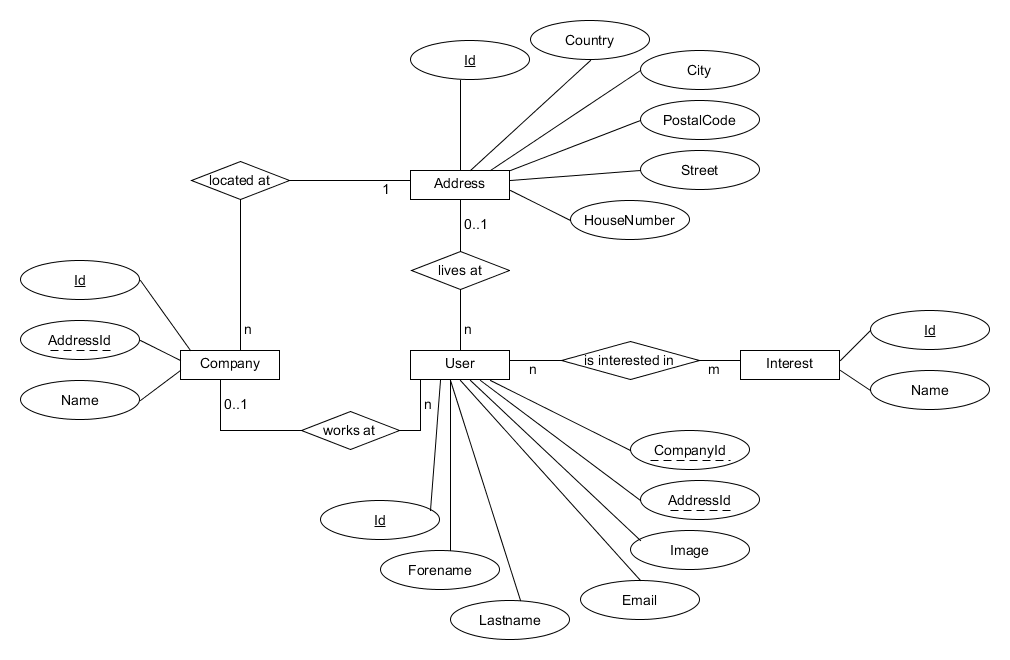
\includegraphics[width=\linewidth]{Images/Projekt_Messe_ERModell2}
	\caption{ER-Modell der Datenbank für die Softwarelösung}
	\label{fig:projektmesseermodell}
\end{figure}

\subsection{Entitäten}
In diesem Abschnitt betrachten wir die Entitäten des ER-Modells und ihre Attribute genauer.

\subsubsection{User}
Die Entität User repräsentiert den Kunden, der seine Daten auf der Messe angegeben hat. Diese Person hat einen Vor- und Nachnamen, Email, Bild, Adresse und eventuell eine Firmenzugehörigkeit. Der Primärschlüssel ist Id, wohingegen AdressId und CompanyId Fremdschlüssel sind.

\subsubsection{Company}
Diese Entität repräsentiert eine Firma, der ein Kunde möglicherweise angehören kann. Sie hat eine Id als Primärschlüssel, einen Namen und eine Adresse mit AddressId als Fremdschlüssel.

\subsubsection{Address}
Die Entität Address hat eine primäre Id, Land, Stadt, Postleitzahl, Straße und Hausnummer.

\subsubsection{Interest}
Eine Interesse hat eine primäre Id und einen Namen.

\subsection{Relationen}

\subsubsection{Company - Address}
Eine Firma hat genau eine Adresse wohingegen an einem Standort auch mehrere Firmen angesiedelt sein können. Dies wird die gezeigte 1:n Relation widergespiegelt. Der Verweise von der Firma auf die Adresse wird mit Hilfe des Fremdschlüssels AddressId gelöst.

\subsubsection{User - Address}
Ein Kunde hat eine oder keine Adresse, wohingegen an einem Ort durchaus mehrere Leute wohnen können. Diese 1:n Relation wird durch den Fremdschlüssel AddressId modelliert.

\subsubsection{User - Company}
Ein Kunde kann Mitarbeiter einer Firma sein, muss es aber nicht und eine Firma kann viele Mitarbeiter haben. Diese 1:n Relation wird durch den Fremdschlüssel CompanyId modelliert.

\subsubsection{User - Interest}
Ein Kunde kann mehrere Interessen haben, aber eine Interesse wie z.B. Reisen kann von vielen Kunden favorisiert werden. Diese n:m Relation wird durch zwei Listen gelöst, wovon sich jeweils eine in der Entität User und Interest befindet.

\newpage
\section{Aufbau und Funktionsweise}
Dieser Abschnitt befasst sich mit dem Aufbau, Architektur und Funktionsweise der Softwarelösung beschrieben mit Hilfe von grafischen Darstellungen mit verschiedenen Diagrammen.

\subsection{Architektur}
\begin{figure}[h]
	\centering
	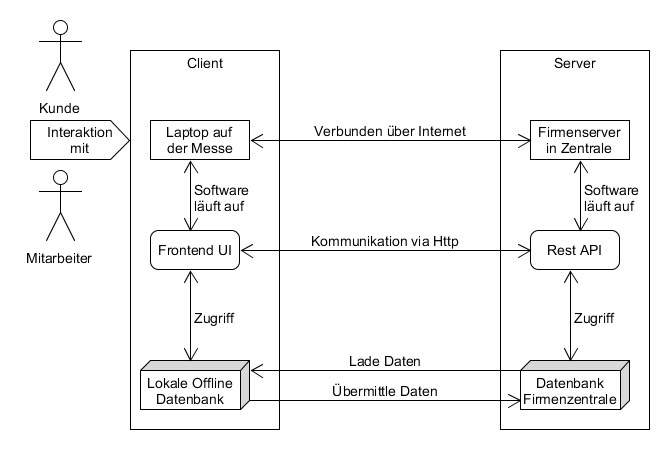
\includegraphics[width=0.8\linewidth]{Images/Projekt_Messe_Architektur}
	\caption{Grafische Darstellung der Architektur}
	\label{fig:projektmessearchitektur}
\end{figure}
Der Aufbau der Softwarelösung ist eine klassische Client-Server-Architektur. Abbildung \ref{fig:projektmessearchitektur} gibt einen Überblick über die beiden Komponenten und ihr Zusammenspiel. 

Der Client befindet sich mit den Mitarbeitern am Messe Stand und ist dort auf den Laptops für die Kunden verfügbar. Dabei handelt es sich um die Frontend UI, die zur Eingabe von Kundendaten und zur Übermittlung an die Firmenserver mit grafische Komponenten dient. Sowohl Kunden als auch Mitarbeiter können den Client bedienen, wobei die Übermittlungsfunktion für Daten lediglich mit Angabe von zuvor registrierten Anmeldedaten benutzt werden kann. Im regulären Betrieb für Kunden befindet sich der Client in einer Art Offline Modus und speichert die Kundendaten in einer lokalen Datenbank ab. Erst nach aktiver Übermittlung an den Firmenserver durch einen Mitarbeiter, werden die Daten zur Firmenzentrale gesendet.

Die Backend Anwendung, eine Rest API, läuft auf den Firmenservern in der Zentrale. Diese wird über das Internet vom Client aus angesteuert, wenn neue Daten durch Mitarbeiter übermittelt werden. Im Gegensatz zur lokalen Client Datenbank, die nur die Daten, des Geräts auf dem diese ausgeführt wird, enthält, sammeln sich in der Datenbank auf dem Firmenserver alle angegebenen Kundendaten an. Zusätzlich werden nach erfolgreicher Übermittlung die Daten vom Client entfernt, um Speicherplatz frei zu machen und Duplikate zu verhindern. Die Mitarbeiter und der Zentrale können im Backend via einer Swagger UI im Browser nach Angabe von validen Anmeldedaten die Kundendaten abfragen.

\newpage
\subsection{USE Case- und Klassen-Diagramme}

\begin{figure}[h]
	\centering
	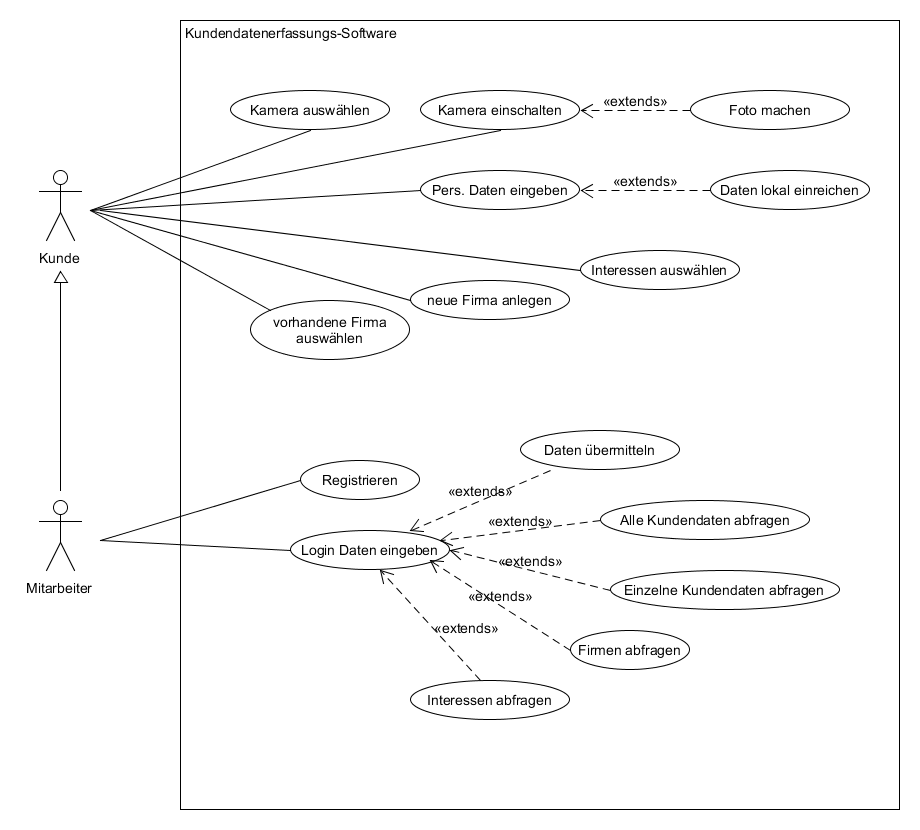
\includegraphics[width=\linewidth]{Images/Projekt_Messe_UseCase2}
	\caption{Use Case Diagramm zur Softwarelösung}
	\label{fig:projektmesseusecase}
\end{figure}

In Abbildung \ref{fig:projektmesseusecase} ist ein Anwendungsfalldiagramm zur Softwarelösung zu sehen. Es gibt zwei Akteure den Kunden und den Mitarbeiter, die verteilt über Frontend UI und Backend Anwendung verschiedene Aktionen durchführen können. Dabei erbt der Mitarbeiter alle Funktionen des Kunden, da dieser auch ohne Angabe von Anmeldedaten alle Aktionen eines Kunden durchführen kann.

\subsubsection{Aktionen eines Kunden}
\begin{itemize}
	\item Kamera auswählen: Mit eine Dropdown Liste kann in der Oberfläche eine Kamera unter all den angeschlossenen gewählt werden. Eine Kamera wird immer als Default ausgewählt sein.
	\item Kamera einschalten: Die ausgewählte Kamera wird eingeschalten und deren Übertragung angezeigt.
	\item Foto machen: Nachdem die Kamera eingeschaltet wurde, kann ein Foto von deren Übertragung gemacht werden.
	\item Persönliche Daten eingeben: Der Kunde kann verschiedene persönliche Daten, wie Name und Anschrift und diversen Textfeldern angeben.
	\item Daten lokal einreichen: Wenn alle notwendigen Daten angegeben wurden, können die Angaben eingereicht und damit lokal gespeichert werden.
	\item Interessen auswählen: Der Kunde kann zwischen verschiedenen vorgegebenen Interessen auswählen und diese per Klick selektieren.
	\item neue Firma anlegen: Wenn von den vorhandenen Firmen keine zusagt, kann eine neue Firma angelegt werden.
	\item Firma auswählen: Der Kunde kann aus verschiedenen angegebenen Firmen eine auswählen.
\end{itemize}

\subsubsection{Aktionen eines Mitarbeiters}
\begin{itemize}
	\item Registrieren: Ein Mitarbeiter kann im Backend neue Anmeldedaten registrieren mit denen er sich später dann in Front- und Backend anmelden kann.
	\item Login Daten eingeben: Der Mitarbeiter kann sowohl im Front- als auch Backend die Anmeldedaten angeben um sich anzumelden.
	\item Daten übermitteln: Nach Angabe von Anmeldedaten kann ein Mitarbeiter die lokal gespeicherten Daten an die Firmenzentrale übermitteln.
	\item Alle Kundendaten abfragen: Ein Mitarbeiter kann nach Angabe von Anmeldedaten im Backend alle Kundendaten abfragen.
	\item Einzelne Kundendaten abfragen: Ein Mitarbeiter kann nach Angabe von Anmeldedaten im Backend einzelne Kundendaten spezifisch abfragen.
	\item Firmen abfragen: Ein Mitarbeiter kann nach Angabe von Anmeldedaten im Backend die Firmen abfragen.
	\item Interessen abfragen: Ein Mitarbeiter kann nach Angabe von Anmeldedaten im Backend die Interessen abfragen.
\end{itemize}
\newpage

\begin{figure}[h]
	\centering
	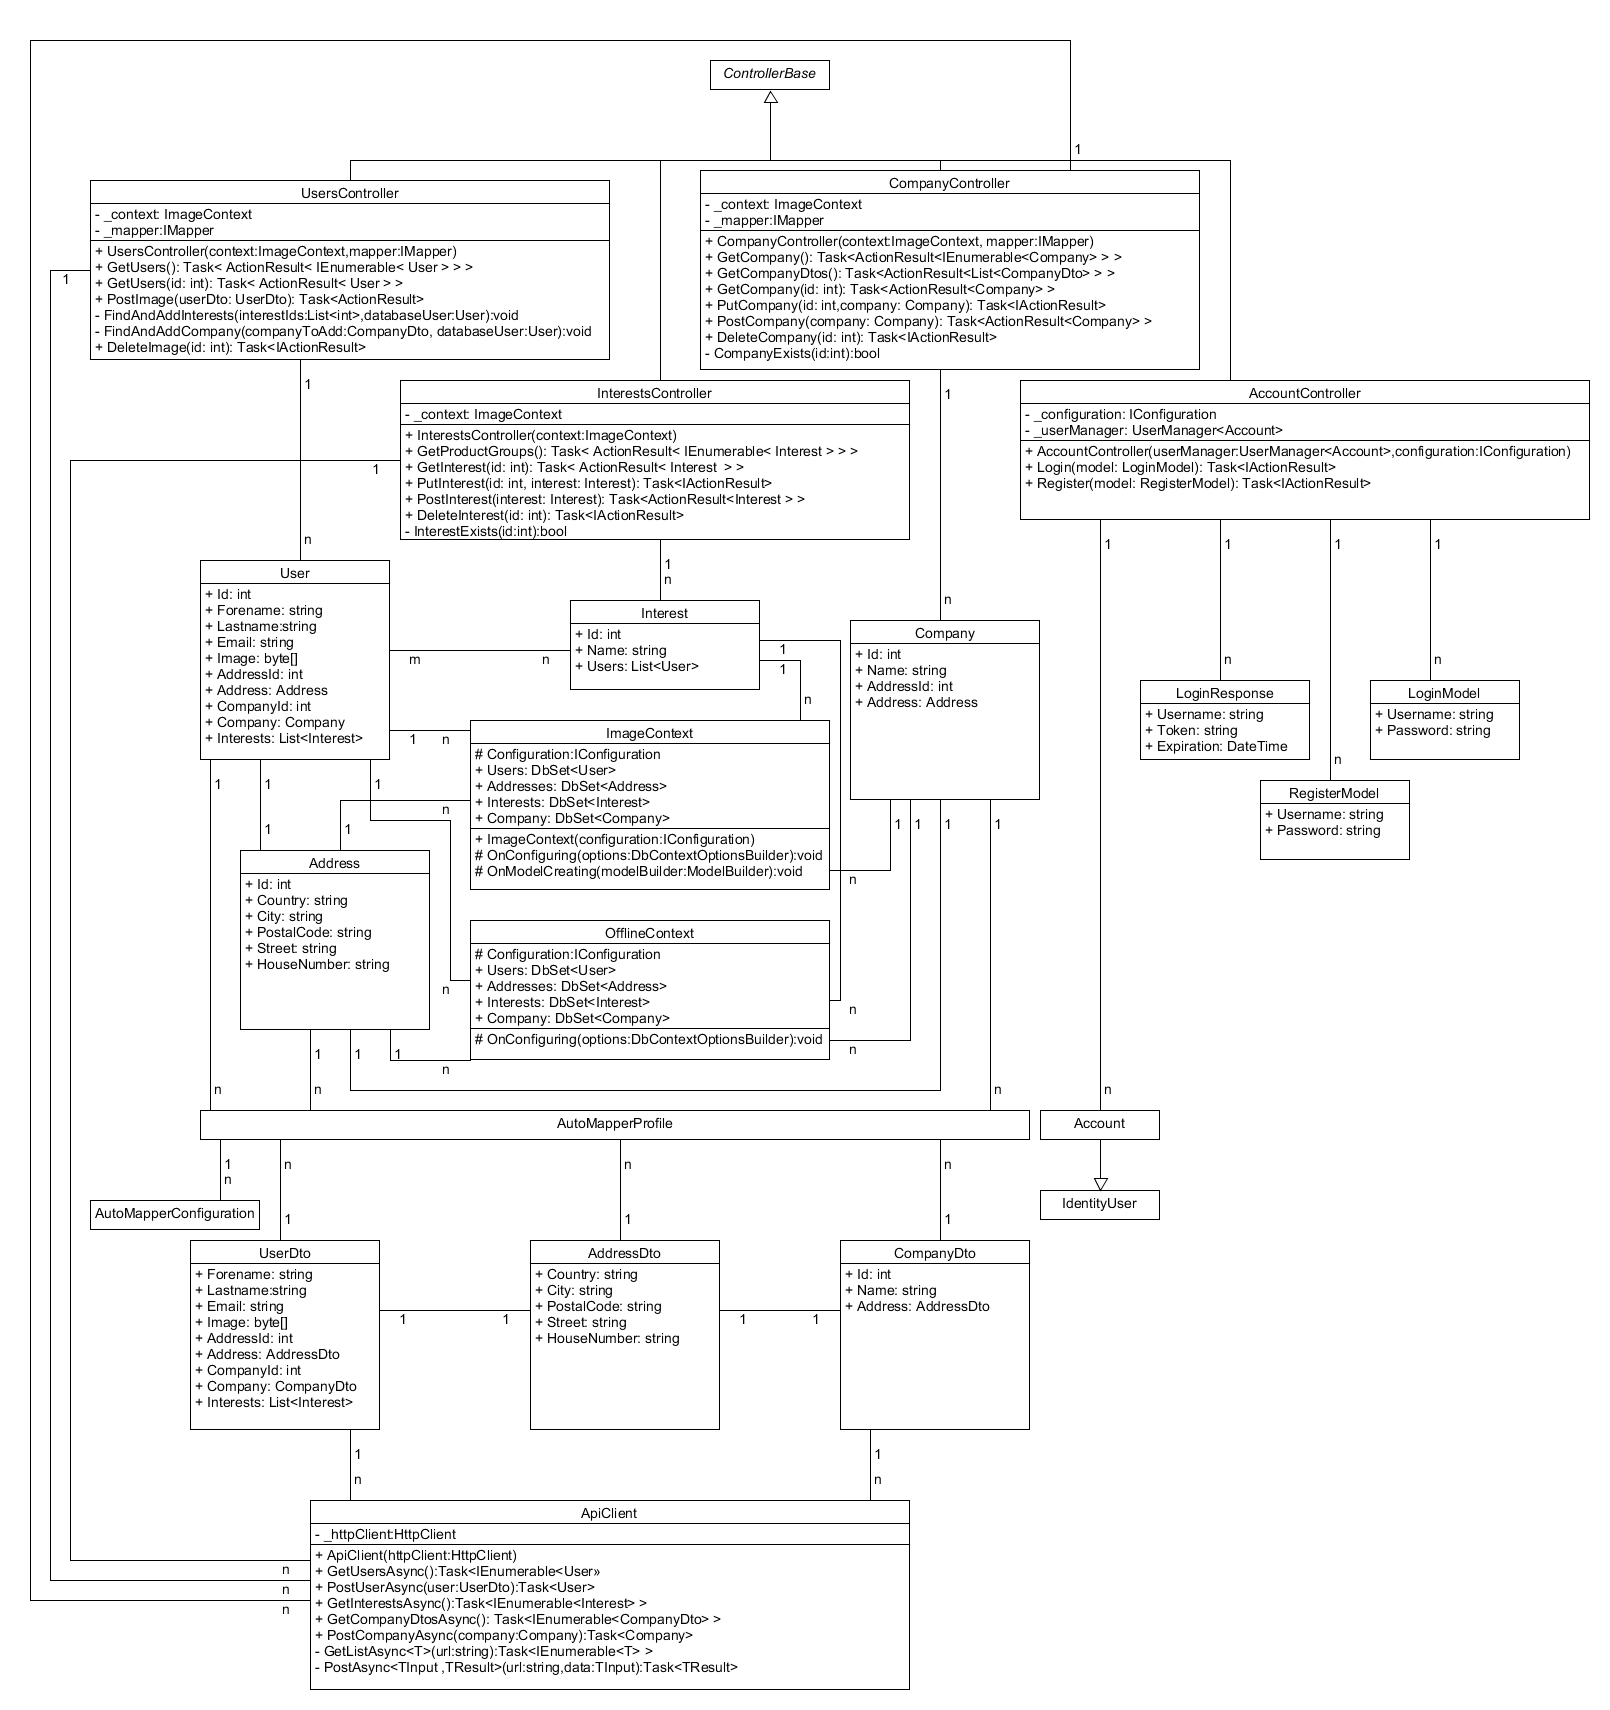
\includegraphics[width=1.1\linewidth]{Images/Projekt_Messe_Class1}
	\caption{Klassen-Diagramm zur Softwarelösung}
	\label{fig:projektmesseclass}
\end{figure}

\subsection{Prerequisites: Bibliotheken und Komponenten}
\subsection{Inbetriebnahme vor Ort}
\subsection{Technische Beschreibung der WebCam Anbindung}
\subsection{Anleitung Bedienung durch den Kunden}
\subsection{Anleitung Datenabruf und Übermittlung}
\subsection{Testszenarien}

